\textit{Les deux premières \namecref{sec:temp-freq} de cette  \namecref{part:param_instant} sont fortement inspirées des propos de \textsc{Cohen} dans son livre \emph{Time frequency analysis} \cite{cohen_time_1995}, chapitre 1 \& 2 }.

\section{Paramètre instantanée dans la cas complexe}\label{sec:temp-freq}


\subsection{Quelques définitions}\label{sec:preli_temp-freq}

Soit $x$ un signal complexe dont $\fou{x}$ ou $\Fou{x}$ est la transformée de Fourier (dont on supposera quelle existe, ici au moins $x\in L^2(\R, \C)$) :
\begin{align*}
	x\ &:\quad \begin{aligned}\R\ &\lr\quad \C \\ x\ &\longmapsto\ x(t)
	\end{aligned}  &  \Fou{x}=\fou{x}\ &:\quad \begin{aligned}\R\ &\lr\qquad\quad \C \\ \nu\ &\longmapsto\ \int_\R x(t)e^{-2\pi i \nu t}dt
	\end{aligned}
\end{align*}
\\
Avant de parlé de fréquences instantanée, il nous faut introduire quelle que définition afin de pouvoir proprement argumenter sa définition.
Tout d'abord, à $x$ sont associées deux densités d'énergie :

\begin{definition}[Densités d'énergie]\label{def:densi_dE}
	La \emph{densité d'énergie} (resp. \emph{spectrale}) du signal $x$, noté $\densit$ (resp. $\densis$), est définie comme :
	\begin{align}\label{eq:densi_dE}
		\densit\ &:\quad \begin{aligned}\R\ &\lr\quad \R^+ \\ t\ &\longmapsto\ \big|x(t)\big|^2 \end{aligned}  
		&
		\densis\ &:\quad \begin{aligned}\R\ &\lr\quad \R^+ \\ \nu\ &\longmapsto\ \big|\fou{x}(\nu)\big|^2 \end{aligned}
	\end{align}
	\\
	La transformée de Fourier étant une isométrie de l'espace $L^2(\R,\C)$, l'\emph{énergie totale} $E(x)={\|x\|_{L^2}}^2$ du signal est indépendante de la représentation de ce dernier (temporelle ou spectrale) :
	\begin{equation}\label{eq:parceval}
		E(x) \defeq  \int_\R \densit(t) dt = \int_\R \densis(\nu) d\nu
	\end{equation}
\end{definition}
\skipl

La première densité, $\densit(t)$, correspond à la puissance (énergie par unité de temps) déployée pour émettre le signal à l'instant $t$ et la seconde, $\densis(\nu)$, à l'énergie associée à la fréquence $\nu$ sur tout le signal. 
\\
Par exemple, si $\ x(t)=e^{2\pi i\nu_0 t}$, alors $\ \fou{x}(t) = \delta(x-\nu_0)$ et on a les densités :
\begin{align*}
	\densit(t) &= 1  &  \densis(\nu) = \delta(\nu-\nu_0)
\end{align*}
On comprend alors que, du point de vu temporel, le signal a été émis avec une puissance régulière, mais le fait que $\densis$ soit un dirac indique que toute l'énergie du signal est concentré en une unique fréquence $\nu_0$.
\\

Les espérances et écart-type on également une interprétation physique :

\begin{definition}[Durée et largeur de bande]\label{def:band-width}
	L'espérance ces densités, pour peu qu'elles existent, sont notées :
	\begin{align*}
		\esp[\densit]{t} &\defeq \int_\R t \big|x(t)\big|^2 dt   &  \esp[\densis]{\nu} &\defeq \int_\R \nu \big|\fou{x}(\nu)\big|^2 d\nu
	\end{align*}
	\\
	Si un signal est localisé temporellement, alors la première espérance/moyenne donne une idée de l'instant d'émission du signal. Si \acontrario, le signal est localisé en fréquence, la seconde espérance peut s'interpréter comme la fréquence ''dominante'' du le signal, ou plus généralement comme sa \emph{fréquence moyenne}. \\
	En particulier, et ce sera important pour la suite, dans le cas des signaux réels, l'espérance de $\densis$ est toujours nulles.
	\\
	On note de même les variances (toujours à condition d'existence) :
	\begin{align*}
		\var[\densit]{t} &\defeq \esp[\densit]{\big(t-\esp[\densit]{t}\big)^2}  &  \var[\densis]{\nu} &\defeq \esp[\densis]{\big(\nu - \esp[\densis]{\nu}\big)^2}\\
		& = \esp[\densit]{t^2} - \esp[\densit]{t}^2  &  &= \esp[\densis]{\nu^2} - \esp[\densis]{\nu}^2
	\end{align*}
	Les écart-types associés sont plus facilement interprétable. Le premier est appelé \emph{durée d'émission} du signal, puisqu'il renseigne l'étalement temporelle du signal ; et le second \emph{largeur de bande (fréquentielle)} puisque, lui, renseigne l'étalement fréquentielle. 
\end{definition}

Ces interprétations reste limité à des cas particulier. Par exemple, et nous y reviendrons, si le support de $\fou{x}$ n'est pas connexe, alors la fréquence moyenne devient beaucoup moins pertinente parce qu'elle à toutes les chances de donnée une fréquence qu'il n'est pas dans le support de $\fou{x}$. Idem pour la largeur de bande qui, dans ce cas, aura plutôt tendance à donnée la distance entre la première et la dernière composante connexe.
\\



\subsection{Amplitude, phase et fréquence instantanée}\label{sec:freq_instant}

Dans le cas des signaux purement complexe, sont très naturellement définit les notions d'\emph{amplitude} et de \emph{phase instantanée} puisqu'elles correspondent respectivement au module et à l'argument de $x$ à l'instant $t$.
\\
Dans le cas le plus simple, où $\ x(t)=e^{2\pi i\nu t + \varphi}$, la fréquence $\nu$ du signal peut s'écrire comme la dérivée :
\[\nu = \frac{1}{2\pi} \frac{d}{dt} (2\pi \nu t + \varphi) = \frac{1}{2\pi} \frac{d}{dt} \arg x(t)\]
\\

Cela invite poser les définitions suivantes :
\begin{definition}
	\'Etant donnée un signal $\ x : t\longmapsto a(t)e^{i\phi(t)}$, on appelle $a$ l'\emph{amplitude instantanée} du signal $x$, $\phi$ sa \emph{phase instantanée} et respectivement $\phi'$ et $\nicefrac{1}{2\pi}\phi'$ son \emph{impulsion} et \emph{fréquence instantanée}.
\end{definition}
\skipl

Pour mieux justifier ces choix de définition, considérons la proposition suivante :

\begin{proposition}\label{prop:mom_freq}
	Si $\densis$ admet une espérance, que $x$ est dérivable et que l'on note :
	alors $a$ et $\phi$ hérite des régularité de $x$ et on a l'égalité (cf. \cref{ann:integ_trick} pour une démonstration) :
	\begin{equation}\label{eq:esp_freq}
		\esp[\densis]{\nu} = \frac{1}{2\pi}\int_\R \phi'(t)\densit(t)dt = \frac{1}{2\pi} \esp[\densit]{\phi'}
	\end{equation}
	De même pour la variance de $\densis$ :
	\begin{equation}\label{eq:var_freq}
		\var[\densis]{\nu} = \frac{1}{4\pi^2}\var[\densit]{(\ln a)'\big.} +\frac{1}{4\pi^2} \var[\densit]{\phi'\big.}
	\end{equation}
\end{proposition}
{\color{white}l} \\
\noindent 

La première égalité \eqref{eq:esp_freq} montre que la moyenne (temporelle) de la fréquence instantanée est égale à la fréquence moyenne (au sens de Fourier). Exprimer ainsi cela parait évident, ce qui est tout à fait rassurant.

Pour la seconde \eqref{eq:var_freq}, on constate deux composantes (qui, par ailleurs, sont des variances purement temporelle). La première ne porte que sur l'amplitude du signal, et inversement, l'amplitude n'apparaît que sur la première. Il donc cohérent que le terme restant, \ie~là où apparaît $\phi'$, porte l'information fréquentielle du signal.
\\



\section{Transformée en signal analytique}

Maintenant que la fréquence instantanée est proprement définie pour les signaux complexes, il nous faut adresser le cas réel.
\\

\subsection{Le problème de signaux réels et comment le résoudre}\label{sec:transfo_SA}

D'abord, du point de vue de l'analyse temps-fréquence, les signaux réels sont problématiques car leur spectre sont à symétrie hermitienne et leur  densité spectrale symétrique :
\begin{align*}
	\forall t\in\R,\ x(t)\in\R \quad &\Lr \quad \forall \nu\in\R,\ \fou{x}(-\nu) = \congu{\fou{x}(\nu)} \\
	&\Lr \quad \forall \nu\in\R,\ \densis(-\nu) = \densis(\nu)
\end{align*}
\skipl \\
Comme mentionné plus haut, cela implique que la fréquence moyenne de tout signal réel est nulle (intégrale d'une fonction impaire). Ce qui, en plus de ne pas être très instructif, n'est pas cohérent avec l'interprétation physique qu'on voudrait faire cette moyenne. Par exemple, si $\densis$ prend la forme ci-dessous (\cref{fig:densi_spec_sym}), alors il serait plus naturelle de demander à ce que la fréquence moyenne se trouve autour de \textbf{1,4}. De même, la largeur de bande spectrale ne correspond plus à l'étalement de chaque gaussienne, mais plutôt à leur espacement.
\\
\begin{figure}[h]\centering
	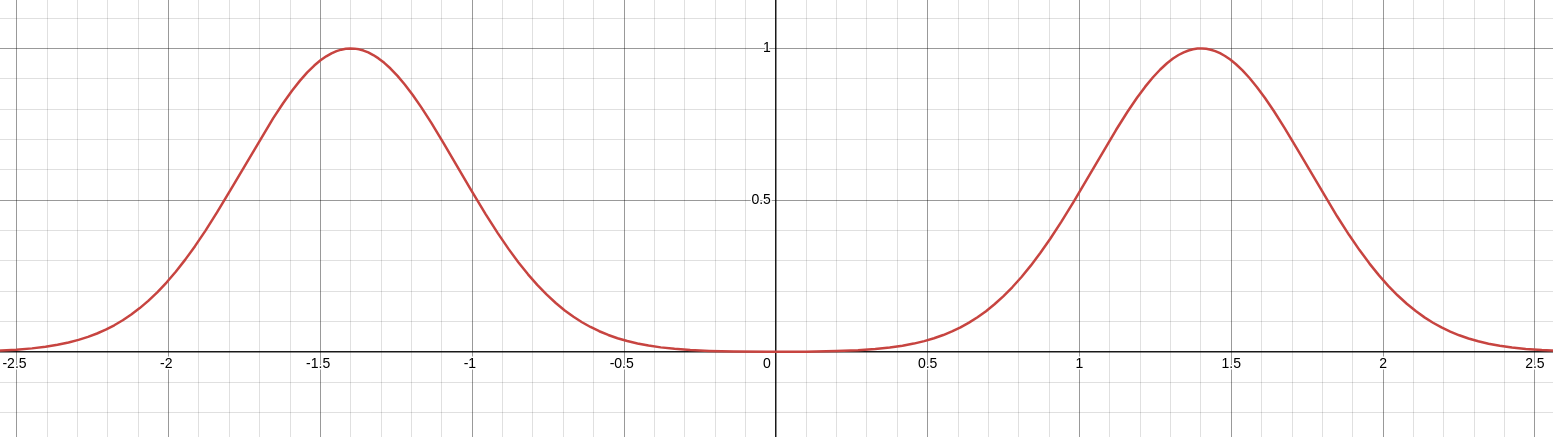
\includegraphics[width=0.9\textwidth]{fig/densi_spec_sym}
	\caption{Exemple de densité spectrale d'un signal réel \textbf{ESP A 1,4}}
	\label{fig:densi_spec_sym}
\end{figure}
\\
Même problème avec la covariance : sachant l'égalité des deux notions de fréquences moyenne (\cref{eq:esp_freq}, \cref{prop:mom_freq}), on peut définir la covariance temps-fréquence d'un signal $x$ par :
\begin{align*}
	\text{Cov}(x) \defeq \text{Cov}\big(t,\phi'(t) \big) 
	&= \esp[\densit]{t\phi'(t)} - \esp[\densit]{t} \esp[\densit]{\phi'(t)} \\
	&= \esp[\densit]{t\phi'(t)} - \esp[\densit]{t} \esp[\densis]{\nu}	
\end{align*}
\\
Ce coefficient est sensé mesurer une corrélation entre l'évolution d'un signal au cours du temps avec ses fréquences. S'il est réel, alors  $\text{Cov}(x)$ sera toujours nulle ; de là à en conclure que la fréquence instantanée de n'importe quel signal (réel) est toujours décorrélée du temps serait, pour le moins, insatisfaisant.
\\

Pour résoudre le problème, une méthode consiste à construire un nouveau signal $\SA{x}$ en supprimant les fréquences négatives de $x$ :
\[\mathcal{F}\big[\SA{x}\big] = 2\one_{\R^+}\fou{x}\]
où $\one_E$ est la fonction indicatrice sur l'ensemble $E$ et où le facteur 2 assure la conservation de l'énergie du signal. Cela mène à la définition :

\begin{definition}[Transformée de Hilbert et en SA]\label{def:transfo_sa&hilbert}
	On appelle \emph{transformé de Hilbert de} $x$, l'application :
	\begin{equation}\label{eq:transfo_Hilb}
		\mathcal{H}[x] :\ \begin{aligned} 
			\R \quad &\lr\qquad\quad \C \\	
			t\quad &\longmapsto\ \frac{1}{\pi}\fint_\R \frac{x(s)}{t-s}ds %=  \frac{1}{\pi}\left(\vpC\right)*x
		\end{aligned}
	\end{equation}
	où l'intégrale barré représente la \emph{valeur principale de Cauchy} (voir \cref{ann:transfo_SA} pour plus de détail) :
	\begin{align*}
		\fint_\R \frac{x(s)}{t-s}ds &\defeq \lim_{\varepsilon\lr0^+} \int_{-\infty}^{-\varepsilon} \frac{\varphi(t)}{t}dt + \int_{+\varepsilon}^{+\infty} \frac{\varphi(t)}{t}dt 
		%\\ &= \int_0^{+\infty} \frac{\varphi(t) - \varphi(-t)}{t}dt
	\end{align*}
	Avec, on définit la \emph{transformée en signal analytique} (SA) de tout signal $x$ comme l'unique application $\SA{x}$ telle que $\ \Fou{\SA{x}\big.}= 2\one_{\R^+}\fou{x}$. Elle est donnée par la formule :
	\begin{equation}\label{eq:transfo_SA}
		\SA{x} :\ \begin{aligned} 
			\R \quad &\lr\qquad\quad \C \\	
			t\quad &\longmapsto\ x(t) + i\mathcal{H}[x](t) %= x(t) + \frac{i}{\pi}\fint_\R \frac{x(s)}{t-s}ds
		\end{aligned}
	\end{equation}
	Plus généralement, tout signal dont le spectre est à support dans $\R^+$ sera dit \emph{analytique}.
\end{definition}
\skipl

Pour mieux comprendre ce que fait la transformation en signal analytique, revenons sur la notion de fréquence instantanée pour les signaux réels.
%Par souci de commodité, plutôt que redéfinir tout le vocabulaire développé plus haut (fréquence moyenne, temps moyen, \etc) pour les signaux réel via la transformation $\mathcal{A}$, dans la suite du mémoire on travaillera directement avec $\SA{x}$. %^(et on verra que c'est essentiel).
\\



\subsection{Interprétabilité de la transformée en SA}\label{sec:Bedrisan&AM-FM}

Pour définir l'amplitude et la phase instantanée d'un signaux réel, on par a nouveau du cas le plus simple. Si $x$ est un signal pur, il va s'écrire :
\[x(t) = a \cos(2\pi\nu t + \varphi),\qquad a,\nu,\varphi\in\R\]
\\
Pour généraliser cette écriture, il suffit donc de poser les amplitude et phase instantanée $a$ et $\phi$ telles que :
\[x(t) = a(t) \cos\big( \phi(t) \big)\]
\\
Contrairement au cas complexe, ici la pair $(a,\phi)$ n'est pas unique et pour contraindre ce choix, on s'appuie sur la transformée $\SA{x}$. Sachant que, dans le cas $x(t)\in\R$, la transformée de Hilbert est à valeur dans $\R$ (intégrale d'une fonction réelle), on a :
\[\SA{x}(t) = a(t)e^{i\phi(t)}\quad \Lr\quad \left\{\begin{aligned}x(t) &= \Re e \SA{x} = a(t) \cos\phi(t) \\ \mathcal{H}[x](t) &= \Im m \SA{x} = a(t) \sin\phi(t)
\end{aligned}\right.\]
\\
D'où la définition :
\begin{definition}[Amplitude et phase instantanée]\label{def:ampli-phase_instant}
	L'\emph{amplitude instantanée} $a_x$ et la \emph{phase instantanée} $\phi_x$ de tout signal $x$ réel sont définies comme étant respectivement l'amplitude et la phase de $\SA{x}$ :
	\begin{align}\label{eq:ampli-phase_instant}
		a_x &= \big|\SA{x}\big|   &   \phi_x &= \arg\big(\SA{x}\big)
	\end{align}
	De même, les \emph{impulsion} et \emph{fréquence instantanée} sont données par $\ \phi'_x\ $ et $\ \nicefrac{1}{2\pi}\phi_x'$.
\end{definition}
\skipl

Si un signal est présenté sous la forme  $\ x=a\cos\phi$, rien n'implique que $a$ et $\phi$ correspondent bel et bien à l'amplitude et la phase instantanée. Si ce n'est pas le cas, c'est que cette décomposition n'est ``pas la bonne'', en cela qu'elles ne s’interprètent pas comme l'on aimerait.
\\
Aussi, quand bien même $x$ peut toujours être écrit comme partie réel de sa transformé en SA, cette écriture n'est nécessairement toujours satisfaisante. Pour le comprendre, détaillons le cas où $x$ s'écrit comme produit de deux signaux pures (\cref{fig:exemple_tSA_1/2}) :
\[x_1(t) = \cos (2\pi\nu_1t)\cos (2\pi\nu_2t)\]

\begin{figure}[h]\centering
	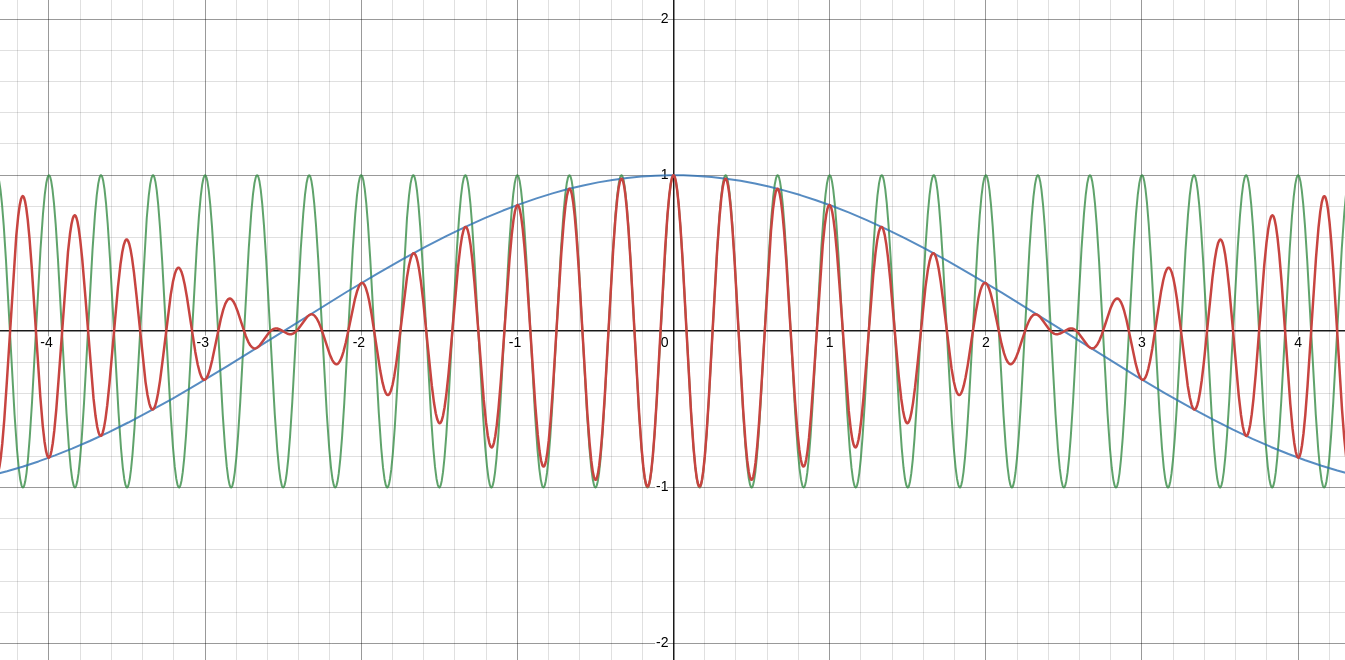
\includegraphics[width=0.48\textwidth]{fig/ex SA - 11.png}
	\hfill
	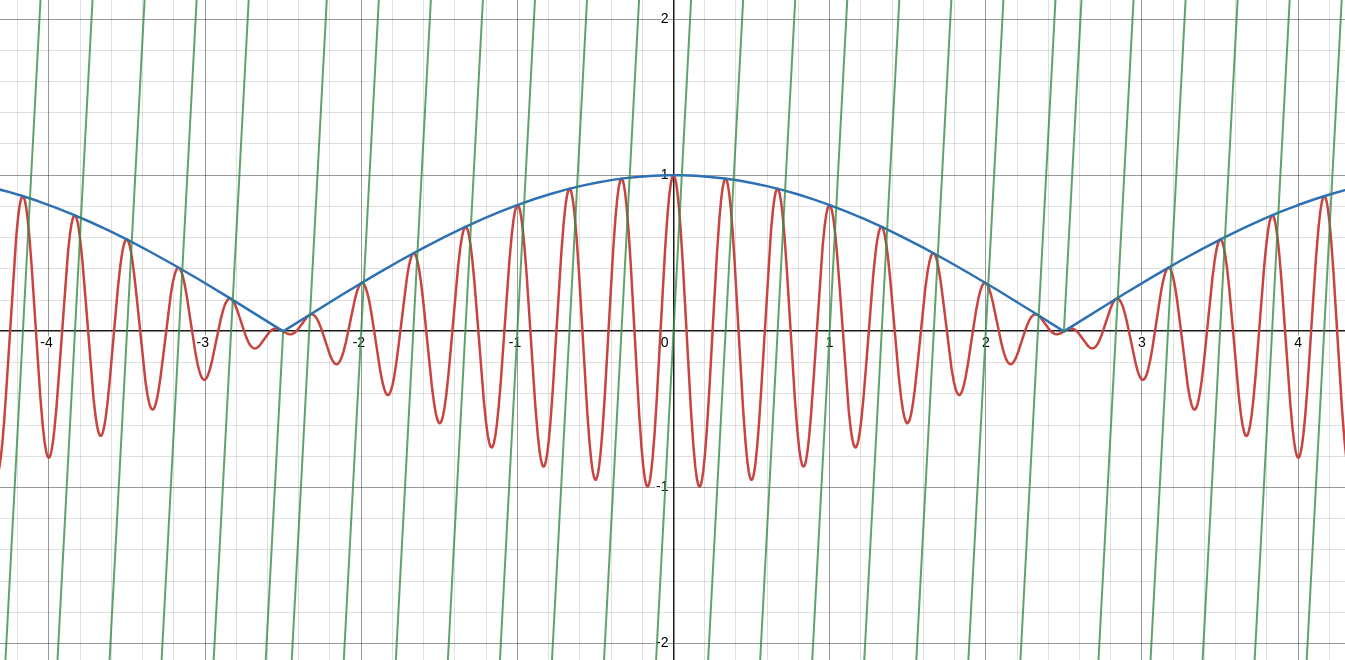
\includegraphics[width=0.48\textwidth]{fig/ex SA - 12.png}
	\caption{Représentation graphique du signal $x$ (rouge) avec $\nu_1=3$ et $\nu_2=0.1$. Sur l'image de gauche, avec signaux de fréquences pures (bleu et vert). Sur l'image de droite, avec son amplitude (bleu) et sa phase instantanée (vert). Les discontinuités de la phase sont dû à l'arrondi à $2\pi$  près de l'argument de $\SA{x_1}$ et à la façon dont il est calculé lorsque le signal s'annule (mise à 0). Voir \href{https://www.desmos.com/calculator/gcedcdfkhr}{ici} pour un graphique dynamique.}
	\label{fig:exemple_tSA_1/2}
\end{figure}

\noindent
On montre sans mal\footnote{\itshape
	$\fou{x}_1$ est donné par 4 Diracs, en ne gardant que ce non nul sur $\R^+$ on obtient le spectre de $\SA{x_1}$ et il reste plus qu'à inverser la transformée de Fourier.}
que si $\ \nu_1\geq\nu_2$, alors la transformée en SA de $x_1$ s'écrit :
\[\SA{x_1} = \cos \left(2\pi\nu_2 t\right) e^{2\i\pi\nu_1 t}\]
\\
Le signal $\SA{x_1}$ n'est ici pas sous forme exponentielle à proprement parler puisque le cosinus peut être négatif (pour s'y ramener, il suffit de passer le cos en valeur absolue et d'ajouter $\pi$ à l'argument lorsque nécessaire) mais l’avantage de cette forme est qu'elle fait clairement apparaître les fréquences $\nu_{1,2}$. En particulier, la fréquence instantanée du signal est la plus grandes des deux fréquences $\nu_1$ et $\nu_2$. La plus petite, elle, se retrouve dans l'amplitude. 
\\
Ce résultat est rassurant en cela qu'il est plus naturel de voir le cosinus de basse fréquence comme modulant celui de haute fréquence que l'inverse comme on le voit sur la première image de la figure \ref{fig:exemple_tSA_1/2}. 
\\
Aussi, en mettant les hautes fréquences du signal dans la fréquence instantanée, on s'assure de limiter les variations de l'amplitude. Cela apporte bien plus de contrainte en terme de décomposition $(a_{x_1},\phi_{x_1})$, en cela qui si l'inverse étant vrai, alors toute les fréquences pourrait être envoyé dans l'amplitude, ce qui laisserait la phase invariante.
\\

Cela étant dit, lorsque l'on fait varier $\nu_1$ et $\nu_2$, le résultat n'est pas toujours si intuitif. C'est notamment le cas lorsque les deux deviennent de plus en plus proche :

\begin{figure}[h]\centering
	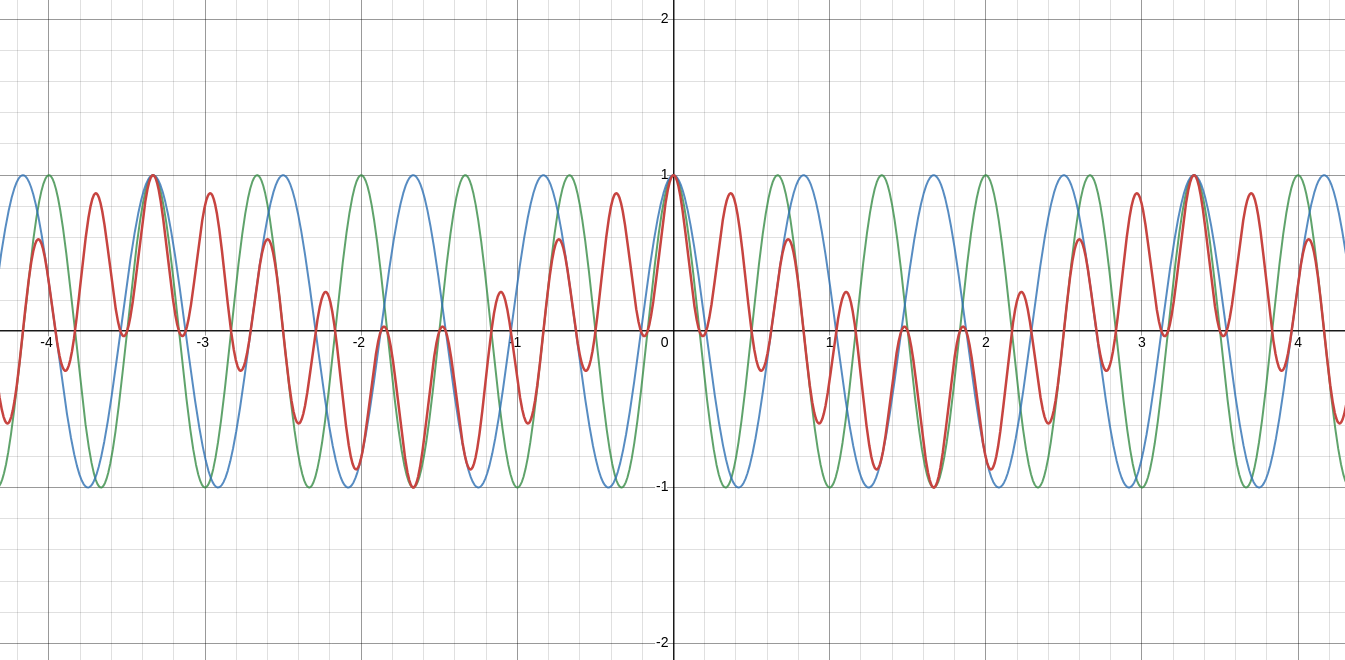
\includegraphics[width=0.48\textwidth]{fig/ex SA - 21.png}\hfill
	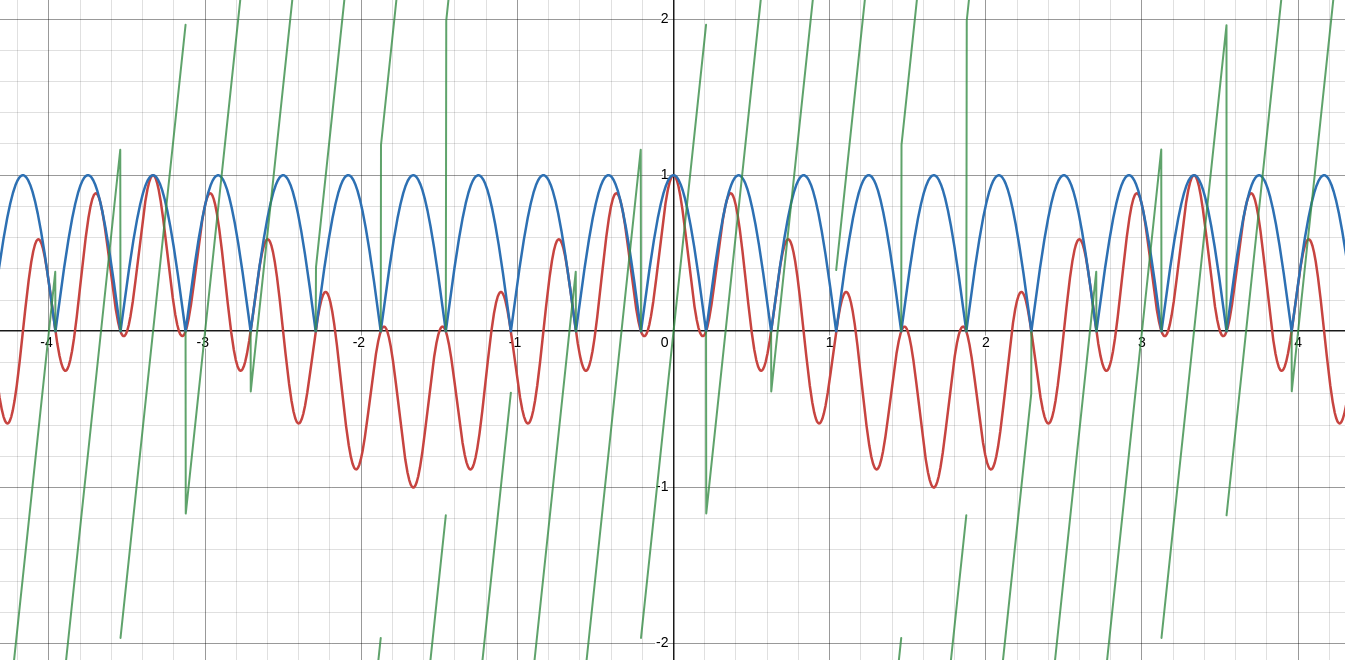
\includegraphics[width=0.48\textwidth]{fig/ex SA - 22.png}
	\caption{Idem que pour la figure \ref{fig:exemple_tSA_1/2} précédente, avec cette fois $\nu_1=1.5$ et $\nu_2=1.3$.}
	\label{fig:exemple_tSA_2/2}
\end{figure}

Pour comprendre pourquoi l'amplitude ne fait pas ce qu'on attendrait d'elle, est introduit le théorème de Bedrosian :

\begin{theoreme}[de Bedrosian]\label{theo:2Bedrosian}
	Dans sa formulation la plus générale, le théorème de Bedrosian énonce que si deux fonctions $f,g\in L^2(\R)$ sont telles l'une des trois assertions suivantes est vraie :
	\begin{itemize}%[label=\textit{\arabic*}. ]
		\item 
		\item $\exists \lambda\in\R^+\ |\ \supp \fou{f} \subset [-\lambda, +\infty[,\ \supp \fou{g} \subset [\lambda, +\infty[$\label{item:1condi_theo2Bedrosian}
		
		\item $\exists \lambda\in\R^+\ |\ \supp \fou{f} \subset ]-\infty, \lambda],\ \supp \fou{g} \subset ]-\infty,-\lambda]$ \label{item:2condi_theo2Bedrosian}
		
		\item $\exists (\lambda_1,\lambda_2)\in \R^+\times\R^+ \setminus\{(0,0)\}\ |\ \supp \fou{f} \subset [-\lambda_1, \lambda_2],\ \supp \fou{g} \subset \R\setminus[-\lambda_2,\lambda_1]$
		
	\end{itemize}
	alors la transformée de Hilbert de leur produit s'écrit (voir \cite{wang_simple_2009} pour une démonstration) :
	\begin{equation}\label{eq:2Bedrosian}
		\hilb{fg} = f\hilb{g}
	\end{equation}
\end{theoreme}

Dans le cas d'un signal réel, suivant la \cref{def:ampli-phase_instant} on peut écrire $\ x=a_x\cos \phi_x$.
Comme $a_x$ et $\cos \phi_x$ sont réelles, seule la troisième condition du théorème de Bedrosian peut être satisfaite pour peu que $\lambda_1=\lambda_2$. Ainsi :

\begin{corollaire}\label{coro:AM-FM}
	Toujours avec les même notations, si $a_x\in L^2(\R)$, $\cos\phi_x\in L^2(\R)$ et qu'il existe $\lambda\in\R^{+_*}$ tel que :
	\begin{equation}\label{eq:condi_AM-FM}
		\supp \Fou{a_x} \subset [-\lambda, \lambda],\quad \supp \Fou{\cos\phi_x} \subset \R\setminus[-\lambda,\lambda]
	\end{equation}
	Alors on a :
	\begin{align}\label{eq:result_AM-FM}
		\hilb{x} &= a_x\hilb{\cos \phi_x}  &  \qquad\qquad&\text{et si }a_x(t)\neq 0,  &  \hilb{\cos \phi_x}(t) = \sin\phi_x(t)
	\end{align}
\end{corollaire}
\skipl

Pour interpréter ce \namecref{coro:AM-FM}, prenons un autre exemple : $\ x_2(t) = a(t)\cos(2\pi \nu_0 t)$. Sa transformé de Fourier est donnée par :
\begin{align*}
	\fou{x}_2(\nu) &= \fou{a}(\nu)*\frac{1}{2}\Big(\delta(\nu-\nu_0) + \delta(\nu+\nu_0)\Big) \\
	&= \frac{1}{2}\Big(\fou{a}(\nu+\nu_0) + \fou{a}(\nu-\nu_0)\Big)
\end{align*}
\\
Graphiquement, la transformé de Fourier de $x_2$ duplique le graphe de $\fou{a}$ en $\pm\nu_0$ et somme les deux. La condition \eqref{eq:condi_AM-FM} du \cref{coro:AM-FM} demande alors que $\nu_0$ soit choisie de telle sorte que :
\[\supp \Fou{a}\subset[-\nu_0, \nu_0]\]
\\
C'est-à-dire qu'il n'y ait pas de chevauchement entre les deux courbes $\ \Gamma_\pm : \nu \longmapsto \fou{a}(\nu\mp\nu_0) $ (voir \cref{fig:alising-ish} ci-dessous). Moralement, cela assure qu'en ne prenant que la partie positive du spectre de $x_2$, l'on ne ramène pas avec une partie de $\fou{a}(\nu+\nu_0)$. Quant bien même cette explication est simpliste puisqu'ici $\phi$ est linaire, on peut voir que le phénomène est finalement très proche de celui d'aliasing.
\\

\begin{figure}[h]\centering
	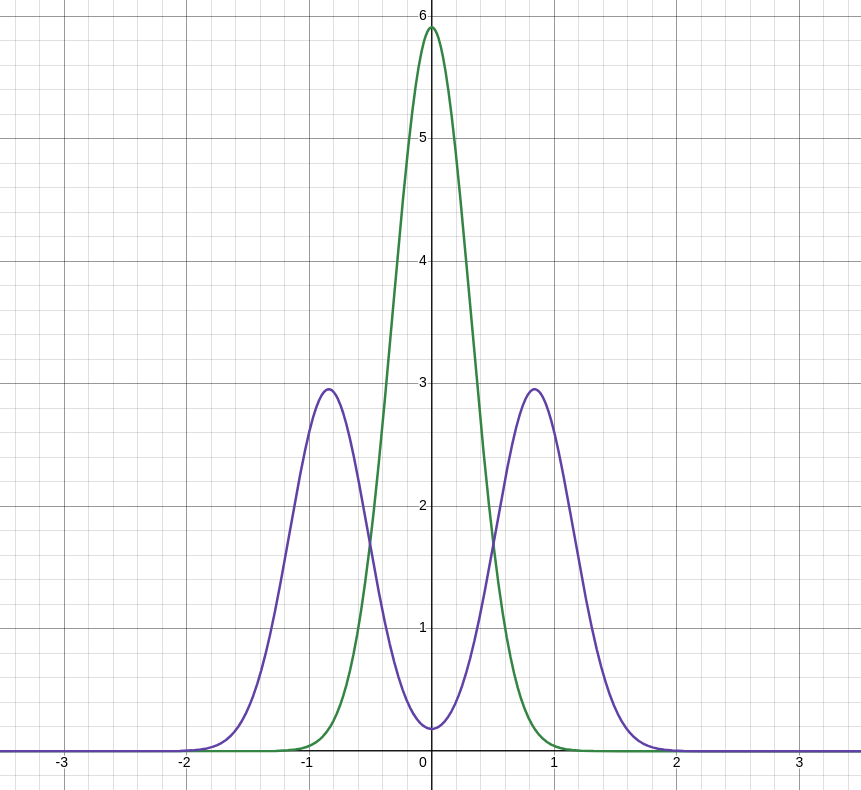
\includegraphics[width=0.45\textwidth]{fig/bedro condi 1.png} 
	\hfill
	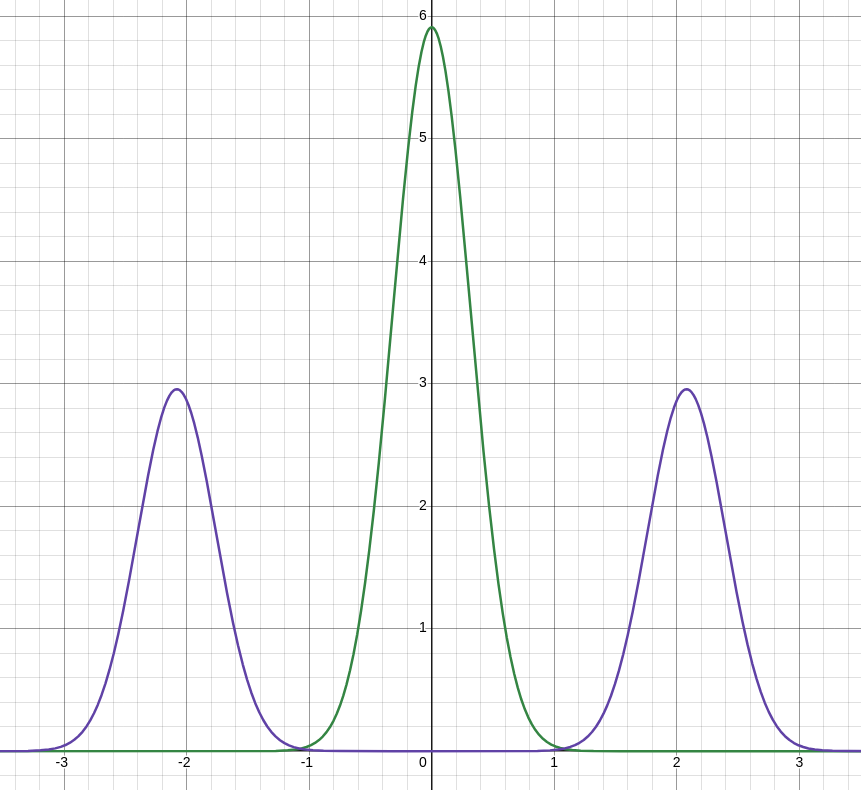
\includegraphics[width=0.45\textwidth]{fig/bedro condi 2.png} 
	\caption{Sur les deux graphiques sont représentés en vert $\fou{a}$ et en violet $\fou{x}_2$. Dans le premier cas l'hypothèse de Bedrosian et respectée mais pas dans le second.}
	\label{fig:alising-ish}
\end{figure}


Pour revenir sur l'exemple $x_1$ précédent, dans la seconde figure \ref{fig:exemple_tSA_2/2}, l'amplitude ne colle plus à l'interprétation que l'on voudrait justement parce que la condition de Bedrosian n'est plus respecter (à savoir $\nu_1\geq 2\nu_2$). 
\\
Formellement, \textbf{JE COMPRENDS TOUJOURS PAS COMMENT CA POSE PROBLEME DANS LA DEFINITON / INTERPRETATION DE $\bf{\SA{x}}$ ! HHHHHH !!!}
\\



\section{Généralisation aux signaux multivariés}\label{sec:sign_multivar}

Maintenant que les paramètres instantanée sont proprement définie pour les cas réel et complexe, qu'en est il des signaux multivariés :

\begin{definition}[Signal multivarié]\label{def:signal_multivar}
	Un \emph{signal multivarié}, ou \emph{$n-$varié}, est un vecteur composé de $n\in\N^*$ signaux $x_i$. Pour $n=2$ (resp.$=3$), on parle de signal \emph{bivarié} (resp. \emph{trivarié}).
	\\
	Dans la continuité de ce qui à été dit dans lplus tôt, dans le cas des signaux réels, on s'intéressera au vecteur composé des transformées en SA (eq. \eqref{eq:transfo_SA}, déf. \ref{def:transfo_sa&hilbert}) des $x_i$.
	%\textbf{Au moins dans toute cette \namecref{sec:sign_multivar}}, un tel signal sera noté :
	%\[\sa{x}(t)\ :\quad \begin{aligned} 
	%	\R\quad &\lr\qquad \C^n \\t\quad &\longmapsto\ \begin{pmatrix} \mathcal{A}[x_1] \\ 
	%		\mathcal{A}[x_2] \\ \vdots \\ \mathcal{A}[x_n] \end{pmatrix}
	%\end{aligned} \]
	\\
	On supposera que chaque composante $x_i$ de $\bf{x}$ aura autant de régularité et de condition d'intégrabilité que nécessaire \textbf{(il vaudra préciser lesquelles éventuellement)}.
\end{definition}

Le fait que $\bf{x}$ soit à valeur dans $\C^n$ impose un choix naturel de d'amplitude instantanée : sa norme. L'on notera alors dans tout la suite (sauf précision) :
\[\forall t\in\R,\qquad 
\bf{x}(t) = a(t)\begin{pmatrix} a_1(t)e^{i\phi_1(t)} \\ a_2(t)e^{i\phi_2(t)} \\ \vdots \\ a_n(t)e^{i\phi_n(t)}
\end{pmatrix} \qquad\text{ avec }\qquad \big\|(a_i)_{1\leq i\leq n}\big\|=1,\quad a\geq 0
%a(t)e^{i\phi(t)}\begin{pmatrix} a_1(t)e^{i\psi_1(t)} \\ a_2(t)e^{i\psi_2(t)} \\ \vdots \\ a_n(t)e^{i\psi_n(t)}\end{pmatrix}
\]
\\
Le choix de la phase instantanée, en revanche, n'est pas plus commode. Si l'on cherche à écrire $\bf{x}$ sous la forme :
\[a(t)e^{i\phi(t)}\begin{pmatrix} a_1(t)e^{i\alpha_1(t)} \\ a_2(t)e^{i\alpha_2(t)} \\ \vdots \\ a_n(t)e^{i\alpha_n(t)}
\end{pmatrix}\]
alors n'importe quel choix de $\phi$ est valable, il suffit que $\ \alpha_i = \phi_i-\phi$.
\\



\subsection{Phase et fréquence instantanée de signal multivarié }\label{sec:param_instant_nvar}

Afin de contraindre ce choix, on s'inspire propriétés de la phase instantanée vu plus tôt pour en déduire deux approches :
\begin{itemize}
	\item D'une part, l'espérance de la fréquence instantanée (ici vu comme dérivée à $2\pi$ près de la phase\footnote{\itshape
		La pertinence de cette définition dans le cas multivarié sera discuté plus loin... \textbf{or is it ? (si oui, dis cref où)}})
	doit donnée la fréquence moyenne au sens de Fourier, eq. \eqref{eq:esp_freq}.
	
	\item D'autre part, les conditions d'interprétation \eqref{eq:condi_AM-FM} de la décomposition $(a_x,\phi_x)$, \cref{coro:AM-FM}, exige que les hautes fréquences du signal se retrouve dans la phase.
\end{itemize}

Pour cela on introduit les notations utiles au cas multivarié :
\begin{definition}[densité d’énergie]\label{def:densi_dE-mv}
	Étant donné un signal multivarié $\bf{x}=(x_i)_{1\leq i\leq n}$, les densités d'énergie de chaque composante $x_i$  sont notées :
	\begin{align}\label{eq:densi_dEi}
		\densit_i\ &:\quad \begin{aligned}\R\ &\lr\quad \R^+ \\ t\ &\longmapsto\ \big|x_i(t)\big|^2 = a(t)^2 a_i(t)^2 \end{aligned}  
		&
		\densis_i\ &:\quad \begin{aligned}\R\ &\lr\quad \R^+ \\ \nu\ &\longmapsto\ \big|\fou{x}_i(\nu)\big|^2 \end{aligned}
	\end{align}
	Et les densités d'énergies associées au signal $\bf{x}$ complet :
	\begin{align}\label{eq:densi_dE-mv}
		\densit\ &:\quad \begin{aligned}\R\ &\lr\quad \R^+ \\ t\ &\longmapsto\ \big\|\bf{x}(t)\big\|^2 = \sum_{i=1}^n \densit_i(t) \end{aligned}  
		&
		\densis\ &:\quad \begin{aligned}\R\ &\lr\quad \R^+ \\ \nu\ &\longmapsto\ \big\|\fou{\bf{x}}(\nu)\big\|^2 = \sum_{i=1}^n \densis_i(t) \end{aligned}	
	\end{align}
\end{definition}
\skipl

La première approche, inspiré de \cite{cano_mathematical_2022} consiste donc de reprendre le ``calculation trick'' \eqref{eq:moment_f}, pour en déduire la fréquence moyenne :
\begin{align*}
	\esp[\densis]{\nu} = \int_\R \nu\densis(\nu)d\nu &= \int_\R \nu\sum_{i=1}^n \densis_i(\nu) d\nu \\
	&= \sum_{i=1}^n\esp[\densis_i]{\nu} \\
	&= \sum_{i=1}^n\frac{1}{2\pi}\int_\R \phi_i'(t)\densit_i(t)dt \\
	&= \frac{1}{2\pi}\int_\R a(t)^2\sum_{i=1}^n\phi_i'(t)a_i(t)^2 dt 
	\\ &= \frac{1}{2\pi} \esp[\densit]{\sum_{i=1}^n \phi_i'{a_i}^2}
\end{align*}
\\
Ce qui mène à une première (potentielle) définition de la phase instantanée :
\begin{equation}\label{eq:phas_inst_v1}
	\phi = \int \sum_{i=1}^n \phi_i'(s){a_i}(s)^2ds 
	= \sum_{i=1}^n \int \phi_i'(s){a_i}(s)^2ds 
	%= \sum_{i=1}^n \esp[\nicefrac{\densit_i}{\densit}]{\phi_i'}
\end{equation}
\\

La seconde approche, fortement inspirée par les travaux de Lilly \& Olhede  \cite{lilly_analysis_2012}, se base sur l'idée de séparation haute/basse fréquences du signal $\bf{x}$. Pour cela, l'on commence par faire apparaître la phase $\phi$ --- pour l'instant inconnue --- en écrivant $\bf{x}$ sous la forme :
\[\forall t\in\R,\qquad \bf{x}(t) = e^{i\phi(t)} e^{-i\phi(t)} \bf{x}(t) \defeq e^{i\phi(t)} \bf{y}(t)\]
\\
Si $\phi$ est bien choisie, alors $\bf{y}$ ne devrait contenir que les informations associées à l'amplitude et la polarisation de $\bf{x}$. Or, la phase doit contenir les hautes fréquences du signal. 
Pour s'en assurer on demande, à l'inverse, que les basses fréquences du signal soient données par $\bf{y}$ en limitant ces variations. Concrètement, $\phi$ doit être choisie de sorte à minimiser la dérivée $\dot{\bf{y}}'$ :
\[\forall t\in\R,\qquad \phi(t) = \argmin{\theta(t)}{\big\|\dot{\bf{y}}(t)\big\|_2}^2 = \argmin{\theta(t)}{\Big\|e^{-i\theta(t)}\big(\dot{\bf{x}}(t) - i\theta(t)'\bf{x}(t)\big)\Big\|_2}^2 = \argmin{\theta(t)}{\big\|\dot{\bf{x}}(t) - i\theta'(t)\bf{x}(t)\big\|_2}^2\]
\\
La contrainte ne dépendant que de la dérivée $\theta'$, on se ramène à :
\[\min_{\theta(t)}{\|\dot{\bf{y}}(t)\|_2}^2 = \min_{\theta'(t)}{\big\|\dot{\bf{x}}(t) - \theta'(t) \bf{x}(t)\big\|_2}^2\]
\\
En rappelant que $\frac{d}{dx}{\big\|f(x)\big\|_2}^2 = 2\Re e\big\langle f(x), f'(x)\big\rangle$, il vient que ce minimum\footnote{\itshape
	L'extremum obtenu est l'unique minimum globale puisque $t\longmapsto \|at + b\|^2$ est strictement convexe pour $a\neq0$.}
est atteint par $\phi'(t)$ à condition que :
\begin{align*}
	\frac{d}{d\phi'}{\big\| \dot{\bf{x}} - i\phi' \bf{x}\big\|_2}^2 = 0 \quad \Llr\quad
	0 &= 2\Re e\left\langle  \dot{\bf{x}} - i\phi' \bf{x} ,  \frac{d}{d\phi'}\big(\dot{\bf{x}} - i\phi' \bf{x}\big)\right\rangle \\
	&= 2\Re e\big\langle  \dot{\bf{x}} - i\phi' \bf{x} ,  - i \bf{x}\big\rangle \\
	&= 2\Re e\Big(i\big\langle  \dot{\bf{x}} ,  \bf{x}\big\rangle\Big) + 2\phi'\Re e\big\langle   \bf{x} ,  \bf{x}\big\rangle\\
	&= -2\Im m\big\langle  \dot{\bf{x}} ,  \bf{x}\big\rangle + 2\phi'{\| \bf{x}\|_2}^2
\end{align*}
Ainsi :
\begin{align}\label{eq:phas_inst_v2}
	\phi' &= \frac{\Im m\big\langle  \dot{\bf{x}} ,  \bf{x}\big\rangle}{{\| \bf{x}\|_2}^2} = \frac{-\Im m\big\langle  \bf{x},  \dot{\bf{x}}\big\rangle}{{\| \bf{x}\|_2}^2}  &  &\text{et}  &  \phi &= -\Im m\int \frac{\big\langle \bf{x}(s) , \dot{\bf{x}}(s) \big\rangle}{\|\bf{x}(s)\|^2} ds
\end{align}
\\
Ce qui, sous forme exponentiel, se réécrit :
\begin{align*}
	-\Im m\frac{\big\langle \bf{x}(t) , \dot{\bf{x}}(t) \big\rangle}{\|\bf{x}(t)\|^2} &= -\Im m\frac{1}{a(t)^2} \sum_{i=1}^n a(t)a_i(t)e^{i\phi_i(t)}\congu{\Big( \big(aa_i\big)'(t) +a(t)a_i(t)i\phi_i'(t)\Big)e^{i\phi_i(t)}} \\
	&= -\Im m\frac{1}{a(t)^2} \sum_{i=1}^n a(t)a_i(t)\big(aa_i\big)'(t) -ia(t)^2a_i(t)^2\phi_i'(t) \\
	&= -\frac{1}{a(t)^2} \sum_{i=1}^n -a(t)^2a_i(t)^2 \phi_i'(t) \\
	&= \sum_{i=1}^n a_i(t)^2 \phi_i'(t)
\end{align*}
Soit la même expression que \eqref{eq:phas_inst_v1} obtenue par le premier raisonnement :
\[-\Im m\int \frac{\big\langle \bf{x}(s) , \dot{\bf{x}}(s) \big\rangle}{\|\bf{x}(s)\|^2} ds = \int \sum_{i=1}^n a_i(s)^2 \phi_i'(s) = \sum_{i=1}^n \int a_i(s)^2 \phi_i'(s)ds\]
\\
Cela justifie la définition :

\begin{definition}[Phase dynalique/instantanée] \label{def:phase_d}
	\'Etant donné un signal $\bf{x}\in \conti{\R}{\C^n}$ quelconque, on appelle \emph{phase instantanée} ou \emph{dynamique} à l'instant $t$ partant du $t_0$, le réel :
	\begin{equation} \label{eq:phase_d}
		\forall t_0, t\in\R, \quad \phased(\bf{x}, t_0,t) \defeq -\int_{t_0}^t \frac{\Im m \big\langle \bf{x}(s) , \dot{\bf{x}}(s) \big\rangle}{\|\bf{x}(s)\|^2} ds =\sum_{i=1}^n \int_{t_0}^t a_i(s)^2 \phi_i'(s)ds
	\end{equation}
	On s'autorisera à omettre les paramètres de $\phased$ lorsque cela ne prête pas à confusion.
\end{definition}
\skipl

Le terme ``dynamique'' viens, entre autre, du fait que dans son cadre d'étude habituelle, la dérivée $\dot{\bf{x}}$ se voit remplacé par un hamiltonien $h\bf{x}$, voir par exemple \cite[sec. 2]{bohm_geometric_2003}, \cite[p.~215]{mukunda_quantum_1993}. En particulier, en mécanique quantique, cet hamiltionien régie l'équation de Schödinger :
\begin{equation}\label{eq:schrodinger}
	i\frac{d \psi(t)}{dt} = h\psi(t)
\end{equation}

Sachant que $\bf{x}$ n'a aucune raison de suivre une telle équation dans notre cas, poser $h = i\frac{d}{dt}$ enlève toute contrainte. On retrouve ainsi, modulo un jeu de convention sur le produit hermitien, la formule \eqref{eq:phase_d} ci-dessus.
\\ Notons enfin qu'une fois la phase dynamique ``extraite'' de $\bf{x}$, le vecteur restant $\bf{y}$ n'a évidement pas de phase dynamique, ce qui se traduit par la formule :
\\



\subsection{Apparition de la phase géométrique}\label{subsub:intro_phaseg}

Pour rentre compte de la pertinence de cette expression, commençons par noter qu'il existe une autre façon standard de définir la phase d'un signal, la \emph{phase totale} :
\begin{equation}\label{eq:phase_t}
	\phaset(\bf{x}, t_0, t) \defeq \arg\big\langle \bf{x}(t), \bf{x}(t_0)\big\rangle
\end{equation}
Il n'est pas clair, dans un cadre générale, comment et pourquoi cela s'interprète bien comme une phase et c'est encore pire lorsque l'on explicite sa valeur :
\begin{align*}
	\phaset(\bf{x},t_0, t) &= \arg \left( \sum_{i=1}^n a_i(t)a_i(t_0)e^{i(\phi_i(t)-\phi_i(t_0))} \right) \\
		&= \phased + \arg \left( \sum_{i=1}^n a_i(t)a_i(t_0)e^{i(\alpha_i(t)-\alpha_i(t_0))} \right)  &  &\text{où } \phi_i = \phased + \alpha_i  \\
		&= \phased + \arctan \left( \sum_{i=1}^n \tan\big( \alpha_i(t)-\alpha_i(t_0) \big) \right)
\end{align*}
\\

Cela étant dit, si $\bf{x}$ est cyclique à une phase près, cette formule fait plus sens. C'est-à-dire lorsque, entre deux instant $t_0$ et $t$ donnés, $\bf{x}$ vérifie :
\[\exists \theta\in\R\ |\quad \bf{x}(t) = e^{i\theta} \bf{x}(t_0)\]
Dès lors, la phase totale donne bien :
\[\arg\big\langle \bf{x}(t), \bf{x}(t_0)\big\rangle = \arg\big\langle e^{i\theta} \bf{x}(t_0), \bf{x}(t_0)\big\rangle = \theta\]
\\
Dans le cas univarié, la phase instantanée vaut également $\theta$, ce qui n'est pas plus le cas dès que $n\geq 2$ (voir \cref{fig:calc_diff_phases}, ci-dessous). Apparaît alors une nouvelle phase qui est dû au caractère multivarié du signal : la phase géométrique introduite au début du mémoire.
\\
\begin{figure}[h]
	
\includegraphics[width=0.6\textwidth]{fig/placeholder}
	\caption{Sur le graphe de gauche, le signal $\bf{x}$ à valeur dans $\R^2$ et dans celui de droite la calcul de la phase dynamique, totale et de leur différence. Résultat tiré des simulation de Le Bihan \etal \cite{le_bihan_modephysiques_2023}}
	\label{fig:calc_diff_phases}
\end{figure}

\textbf{... un peu plus de blabla pour faire transition sur la suite ...}





\begin{annexe}
	
\section{Complément sur l'analyse temps-fréquence} 

\subsection{Un bon moment...}\label{ann:integ_trick}

Pour montrer les formules de la \cref{prop:mom_freq}, on commence par montrer ce que Cohen \cite{cohen_time_1995} appelle les  :

\begin{lemme}[``Calculation tricks''] \label{prop:integ_trick}
	Si le signal est $n$ fois dérivable et que la densité d’énergie spectrale associée $\densis$ admet un moment d'ordre $n$, alors ce moment est donnée par la formule :
	\begin{equation}\label{eq:moment_f}
		\forall n\in\N,\qquad \esp[\densis]{\nu^n} = \left(\frac{i}{2 \pi}\right)^n  \int_\R x(t) \frac{d^n}{dt^n} \congu{x(t)} dt = \left(\frac{i}{2 \pi}\right)^n  \left\langle x, \frac{d^n}{dt^n}x\right\rangle
	\end{equation}
	\\
	Avec les hypothèses analogues, les moments de $\densit$ s'écrivent :
	\begin{equation}\label{eq:moment_t}
		\forall n\in\N,\qquad \esp[\densit]{t^n} = \left(\frac{1}{2i \pi}\right)^n  \int_\R \fou{x}(\nu) \frac{d^n}{dt^n} \congu{\fou{x}(\nu)} dt = \left(\frac{1}{2i \pi}\right)^n  \left\langle \fou{x}, \frac{d^n}{d\nu^n}\fou{x}\right\rangle
	\end{equation}
\end{lemme}


\begin{demo}[du \cref{prop:integ_trick}]
	\`A supposer que les intégrales existes et que le théorème de Fubini s'applique, on a $\forall n\in\N$ :
	\begin{align*}
		\esp[\densis]{\nu^n} = \int_\R \nu^n\densis(\nu) d\nu &= \int_\R \nu^n \fou{x}(\nu)\congu{\fou{x}(\nu)} d\nu \\
		&= \int_\R \nu^n \int_\R x(t)e^{-2i \pi \nu t} dt \int_\R \congu{x(t')}e^{2i \pi \nu t'} dt' d\nu \\
		&= \int_\R \int_\R x(t) \congu{x(t')} \int_\R \nu^n e^{-2i \pi \nu (t-t')} d\nu dt dt' 
	\end{align*}
	Ici, on remarque que :
	\begin{align*}
		\nu^n e^{-2i \pi \nu (t-t')} &= \nu^{n-1}\frac{1}{-2i \pi}\frac{d}{dt}e^{-2i \pi \nu(t-t')} \\
		&= \nu^{n-2}\frac{1}{(-2i \pi)^2}\frac{d^2}{dt^2}e^{-2i \pi \nu(t-t')} \\
		&\ \vdots \\
		&= \frac{1}{(-2i \pi)^n}\frac{d^n}{dt^n}e^{-2i \pi \nu(t-t')}
	\end{align*}
	\\
	
	En jouant sur les ordres d'intégrations, on obtient :
	\begin{align*}
		\esp[\densis]{\nu^n} &= \int_\R \int_\R x(t) \congu{x(t')} \int_\R \nu^n e^{-2i \pi \nu (t-t')} d\nu dt dt'  \\
		&= \int_\R \int_\R x(t) \congu{x(t')} \int_\R \frac{1}{(-2i \pi)^n}\frac{d^n}{dt^n}e^{-2i \pi \nu(t-t')} d\nu\, dt\, dt' \\
		&= \frac{1}{(-2i \pi)^n} \int_\R \int_\R x(t) \congu{x(t')} \frac{d^n}{dt^n}\int_\R e^{-2i \pi \nu(t-t')} d\nu\, dt\, dt' \\
		&= \left(\frac{1}{-2i \pi}\right)^n \int_\R \int_\R x(t) \congu{x(t')} \frac{d^n}{dt^n}\mathcal{F}\big[1\big](t-t') dt\, dt'
	\end{align*}
	La transformée de Fourier de 1 est un dirac, il vient, modulo quelques jeux d'ordre d'intégration :
	\begin{align*}
		\esp[\densis]{\nu^n} &= \left(\frac{1}{-2i \pi}\right)^n \int_\R \int_\R x(t) \congu{x(t')} \frac{d^n}{dt^n}\mathcal{F}\big[1\big](t-t') dt\, dt' \\
		&= \left(\frac{i}{2 \pi}\right)^n \int_\R \int_\R x(t) \congu{x(t')} \frac{d^n}{dt^n}\delta(t-t') dt\, dt' \\
		&= \left(\frac{i}{2 \pi}\right)^n \int_\R x(t) \int_\R \congu{x(t')} \frac{d^n}{dt^n}\delta(t-t') dt' dt \\
		&= \left(\frac{i}{2 \pi}\right)^n \int_\R x(t) \frac{d^n}{dt^n} \int_\R \congu{x(t')} \delta(t-t') dt' dt \\
		&= \left(\frac{i}{2 \pi}\right)^n  \int_\R x(t) \frac{d^n}{dt^n}  \congu{x(t)} dt
	\end{align*}
	%	... a moins que :
\end{demo}
	
\begin{demo}[de la \cref{prop:mom_freq}, \cref{eq:esp_freq}]
	Avec le hypothèses de la \cref{prop:integ_trick} précédente, on a :
	\begin{align*}
		\esp[\densis]{\nu} = \frac{i}{2\pi} \densit(t) \int_\R x(t) \congu{x'(t)} dt &= \frac{i}{2\pi}\int_\R a(t)e^{i\phi(t)}\congu{\big( a'(t)e^{i\phi(t)}+ ia(t)\phi'(t)e^{i\phi(t)} \big)} dt \\
		&= \frac{i}{2\pi}\int_\R a(t)e^{i\phi(t)}\big( a'(t)e^{-i\phi(t)} -ia(t)\phi'(t)e^{-i\phi(t)} \big) dt \\
		&= \frac{i}{2\pi}\int_\R a(t)\big( a'(t)- ia(t)\phi'(t)\big) dt \\
		&= \frac{i}{2\pi}\int_\R a'(t)a(t) dt + \int_\R  \frac{1}{2\pi}\phi'(t)a(t)^2 dt \\
	\end{align*}
	On peut se convaincre que le premier terme doit être nul car l'espérance doit être réelle. On peut s'en assurer par le calcul en notant que c'est l’inégale d'une dérivée :
	\[\int_\R a'(t)a(t) dt = \frac{1}{2} \int_\R \big(a^2\big)'(t) dt = \frac{1}{2}\densit(t)\Big|_{-\infty}^{+\infty} = 0\]
	Ce qui donne bien :
	\[\esp[\densis]{\nu} = \frac{i}{2\pi}\int_\R a'(t)a(t) dt + \int_\R  \frac{1}{2\pi}\phi'(t)a(t)^2 dt = \frac{1}{2\pi}\int_\R \phi'(t)\densit(t) dt\]
\end{demo}


\begin{demo}[de la \cref{prop:mom_freq}, \cref{eq:var_freq}]
	La démonstration est similaire, d'abord, la dérivée seconde de $x$ s'écrit :
	\begin{align*}
		x''(t) &= \frac{d}{dt} \big( a'(t) e^{i\phi(t)} + ia(t)\phi'(t) e^{i\phi(t)} \big) \\
		&= \Big( a''(t) + ia'(t) \phi'(t) + i\big( a'(t)\phi'(t) + a(t)\phi''(t) + ia(t)\phi'(t)\phi'(t) \big) \Big) e^{i\phi(t)} \\
		&= \Big( a''(t) - a(t)\phi'(t)^2 + i\big( 2a'(t)\phi'(t) + a(t)\phi''(t)\big) \Big) e^{i\phi(t)}
	\end{align*}
	de sorte que :
	\begin{align*}
		x(t) \congu{x''(t)} &= a(t) \Big( a''(t) - a(t)\phi'(t)^2 - i\big( 2a'(t)\phi'(t) + a(t)\phi''(t)\big)\Big) \\
		&= a(t)a''(t) - a(t)^2\phi'(t)^2 - i\big( 2a(t)a'(t)\phi'(t) + a(t)^2\phi''(t)\big) \\
		&= a(t)a''(t) - a(t)^2\phi'(t)^2 - i \big( a^2\phi' \big)'(t)
	\end{align*}
	\\
	Ce dont on déduit :
	\begin{align*}
		\esp[\densis]{\nu^2} &= -\frac{1}{4\pi^2} \int_\R x(t) \congu{x''(t)} dt \\
		&= -\frac{1}{4\pi^2} \int_\R a(t)a''(t) - a(t)^2\phi'(t)^2 - i \big( a^2\phi' \big)'(t) dt \\
		&= \frac{1}{4\pi^2} \left( \int_\R a'(t)^2dt + \int_\R a(t)^2\phi'(t)^2 dt - i  a^2(t)\phi'(t)\Big|_{-\infty}^{+\infty} \right)  
			&  &\text{IPP sur le premier membre} \\
		&= \frac{1}{4\pi^2} \left( \int_\R \left(\frac{a'(t)}{a(t)}\right)^2 a(t)^2dt + \int_\R a(t)^2\phi'(t)^2 dt\right) \\
		&= \frac{1}{4\pi^2} \left( \esp[\densit]{\big((\ln a)'\big)^2}  + \esp[\densit]{(\phi')^2\Big.}\right)   &  &\text{car }\ (\ln a)' = \frac{a'}{a}
	\end{align*}
	\\
	Sachant que $\esp[\densit]{(\ln a)'}=0$ (\cf démonstration précédente), il vient :
	\begin{align*}
		\var[\densis]{\nu} &= \esp[\densis]{\nu^2} - \esp[\densis]{\nu}^2 \\
		&= \frac{1}{4\pi^2} \left( \esp[\densit]{\big((\ln a)'\big)^2}  + \esp[\densit]{(\phi')^2\Big.}\right)  - \frac{1}{4\pi^2} \esp[\densit]{\phi'}^2 \\
		&= \frac{1}{4\pi^2} \esp[\densit]{\big((\ln a)'\big)^2} + \frac{1}{4\pi^2}\esp[\densit]{(\ln a)'}^2 + \frac{1}{4\pi^2} \var[\densit]{\phi'\big.} \\
		&= \frac{1}{4\pi^2}\var[\densit]{(\ln a)'\big.} +\frac{1}{4\pi^2} \var[\densit]{\phi'\big.}
	\end{align*}
\end{demo}
\skipl

\subsection{Transformée inverse de la fonction de Heaviside}\label{ann:transfo_SA}

Définissons d'abord proprement la valeur principale de Cauchy :

\begin{definition}[valeur principale de Cauchy]\label{def:vp&Hilb}
	La \emph{valeur principale de Cauchy} est la distribution, notée $\vpC$, définie par dualité :
	\begin{equation}
		\begin{aligned}
			\forall \varphi\in\mathcal{S}(\R),\qquad 
			\left\langle \vpC, \varphi \right\rangle 
			= \fint_0^t \frac{\varphi(t)}{t}dt 
			&\defeq \lim_{\varepsilon\lr0^+} \int_{-\infty}^{-\varepsilon} \frac{\varphi(t)}{t}dt + \int_{+\varepsilon}^{+\infty} \frac{\varphi(t)}{t}dt \\
			&= \int_0^{+\infty} \frac{\varphi(t) - \varphi(-t)}{t}dt
		\end{aligned}
	\end{equation}
	Ici $\mathcal{S}(\R)$ est l’espace de Schwartz des fonctions $C^\infty$ à décroissance rapide et la limite en $\varepsilon$ assure que l'intégrale (impropre) converge bien.
\end{definition}
\skipl

La distribution vp$\frac{1}{x}$ est la valeur principale de la fonction inverse dans le sens où son produit avec l'identité donne 1 $\big(\left\langle id_\R \times \vpC, \varphi \right\rangle = \left\langle \vpC, id_\R \times\varphi \right\rangle=1\big)$ mais avec des propriétés d'intégration supplémentaires. Entre autre :

\begin{propriete}\label{prop:fou2vp}
	La transformée de Fourier de la valeur principale de Cauchy est donnée, au sens des distributions, par :
	\begin{equation}
		\mathcal{F} \left[\vpC \right]= -i \pi\, \sign{} 
	\end{equation}
	Il en découle la transformée de Fourier inverse :
	\begin{equation}
		\mathcal{F}^{-1}\big[ 2\one_{\R^+} \big] = \mathcal{F}^{-1}\big[ 1 + \sign \big] = \delta + \frac{i}{\pi} \vpC
	\end{equation}
\end{propriete}

\begin{demo}
	Par définition, la transformée de Fourier de la valeur principale est telle que,\\ $\forall \varphi\in\mathcal{S}(\R)$ :
	\begin{align*}
		\left\langle \mathcal{F} \left[\vpC \right], \varphi \right\rangle = \left\langle \vpC, \hat{\varphi} \right\rangle 
		&= \fint_\R \frac{\hat{\varphi}(\nu)}{\nu} d\nu \\
		&= \int_0^{+\infty} \frac{\hat{\varphi}(\nu) - \hat{\varphi}(-\nu)}{\nu} d\nu \\
		&= \int_0^{+\infty} \frac{1}{\nu} \left( \int_\R\varphi(t)e^{-2i\pi \nu t}dt - \int_\R\varphi(t)e^{2i\pi \nu t}dt \right)d\nu \\
		&= \int_0^{+\infty} \frac{1}{\nu}\int_\R\varphi(t)\big(e^{-2i\pi \nu t} - e^{2i\pi \nu t}\big)dt\, d\nu \\
		&= \int_0^{+\infty} \frac{1}{\nu}\int_\R-2i\varphi(t)\sin(2\pi \nu t)dt\, d\nu \\
		&= -2i\int_\R\varphi(t)\int_0^{+\infty} \frac{\sin(2\pi \nu t)}{\nu}d\nu\, dt
	\end{align*}
	En posant $u=2\pi\nu t\sign(t)$ (le signe de $t$ assure que l'on ait le même signe dans et hors du sin), on obtient :
	\begin{align*}
		\left\langle \mathcal{F} \left[\vpC \right], \varphi \right\rangle &= -2i\int_\R\varphi(t)\int_0^{+\infty} \sign(t)\frac{\sin(u)}{u}du\, dt \\
		&= -2i\int_\R\varphi(t)\frac{\pi}{2}\sign(t), dt \\
		&= \big\langle -i\pi\sign, \varphi \big\rangle
	\end{align*}
\end{demo}

Finalement, la condition sur le spectre de $\SA{x}$ se traduit bien par :
\begin{align*}
	\Fou{\SA{x}\big.} = 2\one_{\R^+}\fou{x}\quad \Llr\quad \SA{x} &= \iFou{\one_{\R^+}\fou{x}} \\
	&= \iFou{\one_{\R^+}} * \Fou{\fou{x}} \\
	&= \left( \delta + \frac{i}{\pi} \vpC \right) * x \\
	&= x + \frac{i}{\pi} \vpC  * x
\end{align*}
	
\end{annexe}